
\chapter{R\'eseaux de flots et mesures physiques}
\label{ReseauFlotsMesures}
% ----------------------------------------------------------------------------------------------------------------------------------
%		 introduction 
% ----------------------------------------------------------------------------------------------------------------------------------
	Les r\'eseaux \'energ\'etiques ont pour r\^ole de fournir une \'energie \`a des entit\'es consommatrices sans interruption de service. Ces r\'eseaux fonctionnent en courant continu et en alternatif.
\newline
Notre \'etude est limit\'ee au courant alternatif parce que la demande d'\'electricit\'e des \'equipements varie constamment et la quantit\'e d'\'electricit\'e est connue pour chaque \'equipement de ce r\'eseau. 
Notre objectif est de regrouper les \'equipements qui ont la m\^eme source d'alimentation.
Ces sources d'alimentation subissent r\'eguli\`erement des maintenances et le sch\'ema \'electrique n'est pas mis \`a jour, ce qui entraine des probl\`emes dans le syst\`eme de surveillance de ce r\'eseau et aussi dans la planification de nouvelles maintenances.
\newline
Dans ce r\'eseau \'electrique, nous connaissons les liens et les mesures pr\'esentes sur ces liens mais nous ignorons les extr\'emit\'es de ces liens. Notre probl\`eme est d'identifier ces extr\'emit\'es \`a partir des mesures \'electriques. Nous faisons de la {\em d\'ecouverte de topologie}.  
Le mod\`ele propos\'e a \'et\'e \'etabli notamment \`a partir de la description du r\'eseau \'electrique d'un data center d'un op\'erateur t\'el\'ephonique appel\'e {\em Champlan}.
 \newline
Notre chapitre comprend quatre parties. La premi\`ere partie montre la relation entre un r\'eseau \'electrique et un graphe de flots. La seconde partie mod\'elise le r\'eseau de flots et la troisi\`eme partie pr\'esente les travaux existants sur la d\'ecouverte de topologie. 
La derni\`ere partie pr\'esente l'approche retenue pour r\'esoudre notre probl\`eme.

% ----------------------------------------------------------------------------------------------------------------------------------
%		 reseau electrique d'un datacenter : graphe de flots
% ----------------------------------------------------------------------------------------------------------------------------------
	\section{R\'eseau \'electrique d'un data center : un graphe de flots}
		\subsection{Topologie du r\'eseau \'electrique du data center}
			% infrastructure d'un datacenter
Un datacenter ou centre de donn\'ees est un site physique regroupant des installations informatiques interconnect\'ees (serveurs, r\'eseau informatique, syst\`eme de sauvegarde) et une infrastructure \'energ\'etique ad\'equate (un syst\`eme de distribution \'electrique, un commutateur \'electrique, des r\'eserves d'\'energie, des g\'en\'erateurs d\'edi\'es \`a la sauvegarde de donn\'ees, un syst\`eme de ventilation et de refroidissement).
\newline
% caracteristique du reseau electrique
Le r\'eseau \'electrique est le coeur de datacenter car il alimente \`a la fois les infrastructures informatique et \'energ\'etique. Il se compose de quatres entit\'es :
\begin{itemize}
\item {\bf Les sources} : 
ces \'equipements sont les points d'entr\'ee de l'\'electricit\'e dans le datacenter et sont directement rattach\'es au gestionnaire de r\'eseau r\'egional ou national. 
Ils sont de deux types : 
\begin{itemize}
\item Ceux qui alimentent le  r\'eseau en cas de dysfonctionnement du gestionnaire de r\'eseau. Ce sont les accumulateurs, les groupes \'electrog\`enes.
\item Ceux qui transforment l'\'electricit\'e re\c cue du gestionnaire pour des puissances utilisables dans le datacenter. Ce sont les transformateurs basse tension communement appel\'es {\em Transformateur G\'en\'eral Basse Tension (TGBT)}. 
\end{itemize}
G\'en\'eralement, ces deux types d'\'equipements ne fonctionnent pas concomitamment.


\item {\bf Les tableaux} :
aussi appel\'es tableaux de r\'epartition, ce sont des \'equipements passifs dont la fonction est celle de communateur. 
Ils repr\'esentent l'organe centrale de l'installation dans la mesure o\`u ils regroupent tous les circuits \'electriques et syst\`emes de protection vers les baies de serveurs. 
Une baie est une armoire contenant plusieurs serveurs.
Chaque baie poss\`ede un disjoncteur sur ce tableau afin d'interrompre l'alimentation en cas de danger. 
Les tableaux sont consid\'er\'es comme des \'equipements passifs car l'\'electricit\'e qui traverse ces \'equipements a une perte n\'egligeable.   Ces pertes sont les {\em pertes par effets joules}. Un exemple de tableau est pr\'esent\'e dans la figure \`a gauche du tableau \ref{exempleAmoiresTableauxElectriques}. 
%Nous en reparlerons dans la section \ref{pertesEffetsJoules}.

\item {\bf Les baies (ou racks) de serveurs} :
les baies distribuent la puissance n\'ecessaire au fonctionnement de chaque serveur qui lui est rattach\'e. La baie a un r\^ole de multiprise pour tous les serveurs. 
Dans le syst\`eme de supervision \'electrique, les baies sont les consommateurs de l'\'electricit\'e. Elles sont des \'equipements actifs dans le r\'eseau \'electrique.  La figure \`a droite du tableau \ref{exempleAmoiresTableauxElectriques} est un exemple de baie de serveurs. 

\item{\bf Les c\^ables} :
les c\^ables ont pour r\^ole de rattacher les trois entit\'es pr\'ec\'edemment cit\'ees afin de transporter l'\'electricit\'e vers les baies de serveurs. Ils sont caract\'eris\'es par les r\'esistances que nous consid\'erons constantes.
\end{itemize}
% ---- figure exemple amoires ou tableaux electriques et Baie de serveurs 
%\begin{figure}[htb!] 
%\centering
%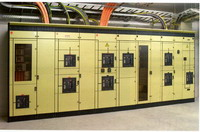
\includegraphics[scale = 0.8]{ReseauFlotsExempleArmoiresTableauxElectriques_okken_PCC.jpg}
%\caption{ \`A gauche :  Tableaux \'electriques entreprise Okken PCC, \`a Droite : baie de serveurs (\lhead{source: news.pixelistes.com}). }
%\label{exempleAmoiresTableauxElectriques}
%\end{figure}
\begin{table}[htb!] 
	\begin{tabular}{cc}
	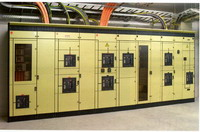
\includegraphics[scale = 1.20]{ReseauFlotsExempleArmoiresTableauxElectriques_okken_PCC.jpg} & 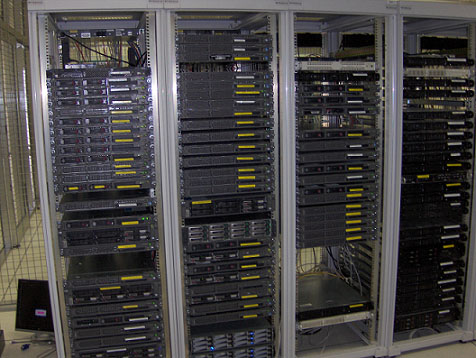
\includegraphics[scale = 0.5]{ReseauFlotsExemple_Baie_serveurs.jpg} \\
	\end{tabular}
	\caption{ Composants \'electriques d'un datacenter. \`A gauche :  tableaux \'electriques Okken PCC, \`a Droite : baie de serveurs (source: news.pixelistes.com). }
\label{exempleAmoiresTableauxElectriques}
%\vspace{-1.5cm}
\end{table}
%\FloatBarrier

% ---- figure exemple amoires et tableaux electriques



		\subsection{R\'eseau \'electrique : un graphe de flots}
			L'\'electricit\'e, achemin\'ee par le gestionnaire de r\'eseau, arrive aux transformateurs basse tension qui g\'en\'eralement fonctionnent en mode triphas\'e.
Ces transformateurs vont convertir la puissance {\em HTA} re\c cue ($20$KVA chez Enedis) en une puissance {\em BT} ($400$KVA) et cette puissance est envoy\'ee sur chaque phase.
Une phase est un canal de transport de courant et 
le courant d'une phase est exprim\'e en fonction du sinus et d'un d\'ecalage de $2\pi/3$ par rapport au courant d'une autre phase.
Chaque phase transporte cette \'energie aux divers tableaux. 
Chaque tableau peut \^etre rattach\'e \`a deux phases pour \'eviter les micro-coupures d'\'electricit\'e. Pendant ces micro-coupures, les accumulateurs et les groupes \'electrog\`enes prennent le relai dans le but d'\'eviter une interruption de service.
Les tableaux sont rattach\'es aux phases et aux baies par des c\^ables \'electriques. 
Chaque \'equipement mesure la quantit\'e d'\'electricit\'e qui le traverse.
Les c\^ables sont unidirectionnels. 
Aucun \'equipement ne s'alimente lui-m\^eme et les \'equipements de m\^eme nature ne sont pas rattach\'es entre eux. Par exemple, il n'existe aucun c\^able entre des tableaux et aucune baie n'alimente une autre baie.
L'\'electricit\'e suit un sens : des sources vers les baies. 
Chaque \'equipement mesure la quantit\'e d'\'electricit\'e qui le traverse. 
 Par convention, ces mesures sont port\'ees par les c\^ables incidents entrants dans chaque \'equipement.
\newline
Notre r\'eseau \'electrique se  mod\'elise avec un r\'eseau de flots dont le graphe est un graphe orient\'e sans circuit {\em Directed Acyclic Graph (DAG)} dans lequel
chaque sommet repr\'esente un \'equipement,
un arc repr\'esente des c\^ables \'electriques et 
 qu'aucun \'equipement ne s'alimente soi-m\^eme (absence de circuits dans le r\'eseau). 
		
{\bf Conclusion} : 
le r\'eseau \'electrique d'un data center comprend des sources, des tableaux, des baies de serveurs et  ils sont tous reli\'es  par des c\^ables \'electriques. Les \'equipements de ce r\'eseau ne s'alimentent pas soi-m\^eme et les \'equipements de m\^eme nature ne poss\`edent pas de c\^ables entre eux. Les c\^ables sont undirectionnels et l'\'electricit\'e a toujours le m\^eme sens : de la source aux baies.
Nous en concluons que la topologie du data center est un {\em graphe orient\'e sans circuit} induit par le sens de la circulation du courant \'electrique sur ces liens. Ainsi ce graphe est la topologie du r\'eseau \'electrique. 

		
% ----------------------------------------------------------------------------------------------------------------------------------
% 		Modelisation du graphe de flots electriques
% ----------------------------------------------------------------------------------------------------------------------------------
	\section{Mod\'elisation du r\'eseau \'electrique du data center}
		\subsection{Description du graphe de flots}
			
Soit $G=(V,A,CAP)$ le graphe orient\'e sans circuit mod\'elisant le r\'eseau \'electrique. 
Chaque sommet de $G$ est soit une source, soit  un tableau ou soit un serveur. 
L'ensemble des sommets $V$ est compos\'e des \'equipements sources $V_S$, interm\'ediaires ou passifs $V_I$ et  charges ou serveurs $V_C$. Il est une union disjointe, deux \`a deux, des partitions $V_C$, $V_I$ et $V_S$ de $V$ de cardinalit\'e $n$ dans laquelle :
\begin{itemize}
	\item Les sommets $V_S$ sont des sommets de degr\'e entrant nul $d^{-} = 0$.
	\item Les sommets $V_I$ sont des sommets de degr\'es entrant et sortant non nuls $d^{-} \ne 0, d^{+} \ne 0$.  
	\item Les sommets $V_C$ sont des sommets de degr\'e sortant nul  $d^{+} = 0$.
\end{itemize}
$$ 
V = V_S \cup V_I \cup V_C ~ et ~ 
V_S \cap V_I =  \emptyset ~ et ~ 
V_S \cap V_C =  \emptyset ~ et ~ 
V_C \cap V_I =  \emptyset
$$
L'ensemble des arcs $A$ mod\'elise $m$ c\^ables \'electriques.
Chaque arc a un flot, une capacit\'e et une r\'esistance consid\'er\'ee constante.
La capacit\'e de chaque arc est fonction de la grandeur associ\'ee \`a cet arc.
\newline
Par convention avec les \'equipes m\'etiers du r\'eseau, nous avons d\'ecid\'e que les arcs incidents entrants dans chaque sommet du graphe portent les mesures des grandeurs physiques.

		\subsection{Grandeurs, flots et contraintes physiques}
			Nous pr\'esentons les grandeurs physiques dans le r\'eseau \'electrique puis d\'efinissons la capacit\'e d'un arc et enfin d\'ecrivons les flots selon chaque grandeur pour un arc donn\'e.

			\subsubsection{Grandeurs physiques}
				Le r\'eseau \'electrique a deux modes de fonctionnement : le mode triphas\'e regroupant les grandeurs $U_{12}, U_{23}, U_{13}, I_{12}, I_{23}, I_{13}$ et le mode monophas\'e regroupant les grandeurs $I,U$. Les autres grandeurs sont communes aux deux syst\`emes (les grandeurs $P, Q, S, cos \phi$). Les symboles
  $U_{12}, U_{23}, U_{13}, U$ sont des tensions,
  $I_{12}, I_{23}, I_{13}, I$ des intensit\'es, 
  $P, Q, S$ des puissances actives, r\'eactives, apparentes respectivement et 
  $cos \phi$ ou $FP$ le facteur de puissance.
\newline 
Une grandeur physique sur un arc est une caract\'eristique physique mesurable selon une unit\'e de mesure. \\
Selon le ph\'enom\`ene physique pris en compte, les grandeurs physiques sont pr\'ed\'efinies. Dans le cas de l'\'electricit\'e, les grandeurs physiques forment l'ensemble \textbf{GP} de cardinalit\'e finie d\'efini comme suit :
\begin{equation}
	GP = \{I, I_{1}, I_{2}, I_{3}, U, U_{12}, U_{23}, U_{13}, P, Q, S, FP \}
\end{equation}
avec le facteur de puissance $FP$ qui d\'esigne le d\'ephasage entre l'intensit\'e ($I$) et la tension ($U$).
\newline
Ces deux modes (triphas\'e et monophas\'e) peuvent fonctionner dans le m\^eme r\'eseau. Cela implique qu'il n'existe qu'un seul sous-ensemble de grandeurs sur un arc, soit des grandeurs monophas\'ees soit des grandeurs triphas\'ees. On note $GP^{a_{i}}$ l'ensemble des grandeurs sur un arc $a_{i} $.
\begin{equation}
	\forall a_{i} \in A, \hspace{0.2cm}  GP^{a_{i}} \subset GP
\end{equation}
On distingue deux types de grandeurs :
\begin{itemize}
	\item Grandeurs \`a diff\'erentiel de potentiel : les tensions. On les note $gp_{ddp} \in \{U_{12}, U_{23}, U_{31}, U\}$.
	\item Grandeurs \`a effet calorique :  l'intensit\'e, la puissance active et r\'eactive. On les note $gp_{cal} \in \{ P, I_{1}, I_{2}, I_{3}, Q\}$.
\end{itemize} 
			\subsubsection{Capacit\'e d'un arc}
				Soit un arc $a_{i} \in A$ et $GP^{a_{i}} \in GP$ l'ensemble des grandeurs physiques associ\'ees \`a l'arc  $a_{i}$.
La  capacit\'e d'un arc $a_{i}$ est une fonction $Cap_{a_{i}}$ qui, pour chaque grandeur physique $GP^{a_{i}}$ associe une valeur r\'eelle positive $\R^{+}$.
\begin{equation}
	Cap_{a_{i}}: GP^{a_{i}} \rightarrow \R^{+}
\end{equation}
Le  vecteur $CAP$ contient les capacit\'es pour chaque grandeur et chaque arc.
\begin{equation}
	CAP = (Cap_{a}[x])_{ a \in A, x \in GP^{a} }
\end{equation}
			\subsubsection{ Description d'un flot physique}
				Les mesures physiques sont des valeurs de ces grandeurs.
%Le vecteur de mesures $gp(a, gp_{a})$ est de norme $T^{a,gp_{a}}$ associ\'e \`a l'arc $a$ et le i$^{ieme}$ \'el\'ement pris dans cette s\'erie de mesures est  $gp(a,gp_{a}, i)$. 
Le vecteur de mesures $gp_{a}^{x}$ de norme $T^{a,x}$ (c'est-\`a-dire le nombre de valeurs associ\'ees \`a une grandeur dans une s\'erie temporelle) est une s\'erie de mesures associ\'ee \`a l'arc $a$ et \`a la grandeur $x \in  GP^{a}$ dont le i$^{ieme}$ \'el\'ement est  $gp_{a}^{x}[i]$.
Le vecteur $gp_{a}^{x}$ associ\'e \`a la grandeur $x \in GP^{a}$ et \`a l'arc $a \in A$ est d\'efini comme suit :
\begin{equation}
	gp_{a}^{x} = ( gp_{a}^{x}[t] )_{0 < t < T^{a, x} }
\end{equation}
avec $ gp_{a}^{x}[t] \in \R^{+}$ et $ t \in \N^{+}$.
\begin{remark}
\label{remarque} 
Soient  $gp_{a}^{x}[t]$ le t$^{ieme}$ \'el\'ement de la s\'erie temporelle de la grandeur $x \in GP^{a}$ et $a, a'$ deux  arcs distincts.
\begin{itemize}
	\item  $gp_{a}^{x}[t]$ et  $gp_{a}^{y}[t]$, pour $x, y \in GP^{a}$ sont prises aux m\^emes instants.
	\item  pour $x\in GP^{a} \cap GP^{a'}$,  $gp_{a}^{x}[t]$ et  $gp_{a'}^{x}[t]$  sont prises \`a des instants diff\'erents.
\end{itemize}
\end{remark}
Certaines valeurs de $ gp_{a}^{x}$ sont ind\'efinies ou \'erron\'ees dans certains cas.

			\subsubsection{ Contraintes sur les flots}
				 \label{reglesLocales}
Un flot  $gp_{a}^{x}[t]$ est admissible s'il respecte, pour chaque arc $a \in A$ travers\'e, la contrainte ci-dessous:
\begin{equation}
	0 \le  gp_{a}^{x}[t] \le Cap_{a}[x]
\end{equation}	
avec $Cap_{a}$ la capacit\'e de l'arc $a$ pour la grandeur $x \in GP^{a}$.
\newline
Un flot est une fonction qui prend en entr\'ees 
un arc $a$, 
une grandeur $x \in GP^{a}$, 
un vecteur $gp_{a}^{x}$ associ\'e \`a la grandeur $x$ de l'arc $a$, 
un facteur de puissance $cos \phi$ ou $FP$ associ\'e  \`a l'arc $a$
et retourne un vecteur d\'efini comme suit :
\begin{equation}
	flo(a,x,gp_{a}^{x}) = f(a, x, r, cos \phi, gp_{a}^{x}) =
	\begin{cases}
		 \frac{  gp_{a}^{x} }{r \times cos \phi}, x \in gp_{ddp} \\
		 gp_{a}^{x} , x \in gp_{cal}
	\end{cases}
\end{equation}
avec $r$ la r\'esistance du c\^able, FP ou cos $\phi$ le facteur de puissance.
\newline
Une valeur $flo_{t}(a,x,gp_{a}^{x})$ de $flo(a,x,gp_{a}^{x})$ s'obtient \`a un indice $t < T^{a, x}$ donn\'e et se d\'efinit comme suit : 
\begin{equation}
	flo_t(a,x,gp_{a}^{x}) = f(a, x, r, cos \phi, gp_{a}^{x}) =
	\begin{cases}
		 \frac{  gp_{a}^{x}(t) }{r \times cos \phi}, x \in gp_{ddp} \\
		 gp_{a}^{x}(t) , x \in gp_{cal}
	\end{cases}
\end{equation}
Soient $a \in A$ un arc et $x \in GP^{a}$ une grandeur li\'ee \`a l'arc $a$.
L'ensemble des arcs incidents \`a $a$ ayant la m\^eme extr\'emit\'e initiale que $a$ est not\'e  $succ(a)$ et 
 l'ensemble des arcs incidents \`a $a$ ayant la m\^eme extr\'emit\'e finale que $a$ est not\'e $pred(a)$.
 Tous les \'el\'ements de $succ(a)$ et $pred(a)$ ont les m\^emes grandeurs physiques. 
 \newline
La fonction $flo$ doit respecter la contrainte de la loi de conservation $R$ \cite{loiDeConservation}. La loi de  conservation $R$ ne s'applique qu'avec les grandeurs \`a effet calorique $gp_{cal} \in GP$ et se d\'efinit  comme suit :
\begin{enumerate}
		\item 
			\begin{equation}
				\sum_{a_{j} \in pred(a)} flo_t(a_{j},x,gp_{a_{j}}^{x}) = \sum_{a_{k} \in succ(a)} flo_t(a_{k},x,gp_{a_{k}}^{x}) + \epsilon 
			\end{equation}
		avec $\epsilon$ les pertes par effets joules. Cette \'equation est la loi de conservation ou de Kirchhoff

%		\item L'extr\'emit\'e finale de $a$ est un puits ou noeud consommateur
%			\begin{equation}
%				si~ succ(a) = \emptyset ~ alors ~ \sum_{a_{j} \in pred(a)} flo_t(a,x,gp_{a}^{x}) \ge 0 
%			\end{equation}	
%		\item L'extr\'emit\'e initiale de $a$ est une source ou noeud source
%			\begin{equation}
%				si ~ pred(a) = \emptyset ~ alors ~ \sum_{a_{j} \in succ(a)} flo_t(a,x, gp_{a}^{x}) \ge 0 
%			\end{equation}	
\end{enumerate}


%Soient 2 arcs $a_{i}, a_{j}$ ayant une extr\'emit\'e en commun, et une grandeur physique $gp_{a} \in GP$.\\
%Un flot $flo$ est une fonction qui prend en entr\'ee un arc et une grandeur physique et qui fournit une valeur r\'eelle en sortie. 
%Le flot d\'epend des caract\'eristiques  de l'arc (r\'esistance, cos $\phi$) et se d\'efinit ainsi:
%\begin{equation}
%	flo(a,gp_{a}^{x}) = f(a, r, cos \phi, gp_{a}^{x}) =
%	\begin{cases}
%		 \frac{  gp_{a}^{x} }{r \times cos \phi}, x \in gp_{ddp} \\
%		 gp_{a}^{x} , x \in gp_{cal}
%	\end{cases}
%\end{equation}
%avec $x \in GP^{a}$, $r$ la r\'esistance du c\^able, FP ou cos $\phi$ le facteur de puissance. \\
%Le vecteur de flot $flo(a,gp_{a}^{x})$ est de norme $T^{a,x}$.\\
%Une valeur de $flo(a,gp_{a}^{x})$ s'obtient \`a un indice $t < T^{a, x}$ donn\'e c'est-\`a-dire $flo_{t}(a,gp_{a}^{x})$
%\begin{equation}
%	flo_{t}(a, gp_{a}^{x}) = f[a, r, cos \phi, gp_{a}^{x}, t] =
%	\begin{cases}
%		 \frac{  gp_{a}^{x}[t] }{r \times cos \phi}, gp \in \{U, U_{12}, U_{23}, U_{13}  \} \\
%		 gp_{a}^{x}[t] , gp \in \{P, Q, I, I_{1}, I_{2}, I_{3}  \}
%	\end{cases}
%\end{equation}
%La loi de conservation aussi nomm\'ee  \textbf{r\`egles locales $R$} ne s'applique qu'avec les grandeurs \`a effet calorique $gp_{cal} \in GP$ et se d\'efinisse  comme suit:
%	\begin{enumerate}
%		\item 
%			\begin{equation}
%				\forall a_{i} \in A_{gp},  \sum_{a_{j} \in P(a_{i})} flo(a_{j},gp_{a_{j}}^{x}) = \sum_{a_{k} \in S( a_{i} )} flo(a_{k},gp_{a_{k}}^{x}) + \epsilon 
%			\end{equation}
%		avec $\epsilon$ les pertes par effets joules. Cette \'equation est la loi de conservation ou de Kirchhoff
%
%		\item l'extr\'emit\'e finale de $a_{i}$ est un puits ou noeud consommateur
%			\begin{equation}
%				si \hspace{0,1cm} S( a_{i} ) = \emptyset \hspace{0,1 cm} alors \hspace{0,1cm} \forall a_{i} \in A_{gp}, \sum_{a_{j} \in S(a_{i})} flo(a_{j},gp_{a_{j}}^{x}) \ge 0 
%			\end{equation}	
%		\item l'extr\'emit\'e initiale de $a_{i}$ est une source ou noeud source
%			\begin{equation}
%				si \hspace{0,1cm} P( a_{i} ) = \emptyset \hspace{0,1cm} alors  \hspace{0,1cm} \sum_{a_{j} \in P(a_{i})} flo(a_{j}, gp_{a_{j}}^{x}) \ge 0 
%			\end{equation}	
%	\end{enumerate}
%avec $ S(a_{i}) = \{a_{j}: a_{i}^{-} = a_{j}^{-}   \}$ l'ensemble des arcs ayant la m\^eme extr\'emit\'e initiale que $a_{i}$ et 
% $ P(a_{i}) = \{a_{j}: a_{i}^{+} = a_{j}^{+}   \}$  l'ensemble des arcs ayant la m\^eme extr\'emit\'e  finale que $a_{i}$.
			\subsubsection{Description de Verif-correl}
				\label{VerifCorrel}
La fonction $Verif-correl$ d\'etermine le sous-ensemble d'arcs entrants et sortants d'un sommet du r\'eseau \'electrique en se basant sur les mesures physiques et les lois de conservation $R$ d\'efinies dans le paragraphe \ref{reglesLocales}. 
\newline
Soit $S \subset A$ l'ensemble  fini d'arcs incidents \`a un sommet  $v \in V$ et 
$x \in GP$ une grandeur physique 
telle que chaque arc $a \in S$ a un flot $gp_{a}^{x}$.
Nous partitionnons $S$ en deux sous-ensembles $S_1$ et $S_2$ tels que $S_1 \cap S_2  = \emptyset$.
\newline
La fonction $Verif-correl$ est bool\'eenne, prend en param\`etres $S_1$, $S_2$ et une grandeur $x$. 
Elle retourne $1$ si :
\begin{itemize}
	\item $S_1$ est l'ensemble des arcs entrants du sommet $v$.
	\item $S_2$ est l'ensemble des arcs sortants du sommet $v$.
\end{itemize} 
Si les lois $R$ ne sont pas v\'erifi\'ees alors $Verif-correl$ retourne $0$.
$$
Verif-correl(S_1, S_2, x) = 1 \Leftrightarrow  \sum_{ a_i \in S_1} gp_{a_i}^{x}(t) - \sum_{a_ j\in S_2} gp_{a_j}^{x}(t)  \le \epsilon 
$$
En effet, consid\'erons $t$ un instant de temps et 
		$diff(t) =  \sum_{ a_i \in S_1} gp_{a_i}^{x}(t) - \sum_{a_ j\in S_2} gp_{a_j}^{x}(t)$ 
la diff\'erence entre les flots entrants et sortants \`a un instant $t$.
La diff\'erence $diff(t)$ doit toujours \^etre inf\'erieure aux pertes par Effet Joule $\epsilon$ quel que soit l'instant $t$. 
\newline
Nous d\'ecidons que la fonction $Verif-Correl$ retourne $0$ si 
le nombre de diff\'erences $diff(t)$ sup\'erieure \`a $\epsilon$ est sup\'erieur \`a un seuil (choisi \`a $10\%$).
%la moyenne des diff\'erences $\frac{\sum_{t=0}^{T} diff(t)}{T}$  est sup\'erieure \`a un seuil (choisi \`a $10\%$).
\newline


Nous consid\'erons, dans la suite du rapport, que la {\em d\'ecision de $Verif-correl$ est toujours exacte}. Cela signifie que 
si $Verif-correl(S1, S2, x) = 0$ alors les arcs de $S$ ne partagent pas un sommet de $V$.
Cependant, dans la pratique, nous n'utilisons pas cette fonction pour d\'eterminer la topologie car pour un sommet $v$ de la topologie ayant un ensemble d'arcs $S_v$, nous devons  tester de l'ordre de $2^{|S_{v}|}$ bipartitions dans le pire des cas pour obtenir la bonne bipartition et cela est impossible pour $S_{v}$ tr\`es grand. 

%			 \subsubsection{ Influence des pertes par effets joules} 
%			 	%epsilon est le taux min des pertes par effets joules pour lequel l'oracle ne comet pas d'erreurs.
% EJ ce sont les pertes par effet joules dans le reseau.

% DECISION : ABANDON DE CE PARAGRAPHE car utilise les algorithmes de couvertures
Nous consid\'erons que le r\'eseau \'electrique modelis\'e par un DAG $G$ est connu.
Nous \'etudions l'\'evolution du pourcentage minimum des pertes par effets joules not\'ee $\epsilon$ en fonction des partitions coh\'erente propos\'ee par  {\em Verif-correl}.
Nous d\'efinissons la {\em similarit\'e} comme \'etant le pourcentage d'arcs de $A$ bien pr\'edits par $Verif-correl$.
Nous r\'ealisons deux exp\'eriences: 
\begin{itemize}
\item La premi\`ere exp\'erience consiste \`a g\'en\'erer des mesures de flots de divers graphes en faisant varier, de $0$ \`a $1$ par pas de $0.125$, les pertes par effets joules $EJ$ tout en fixant la variable $\epsilon$. Nous ex\'ecutons l'algorithme de couverture sur diff\'erents graphes, chaque graphe ayant un $EJ \in [0,1]$. Nous \'etudions l'\'evolution de la  similarit\'e en fonction de pertes joules $EJ$. 

\item La deuxi\`eme exp\'erience consiste \`a faire varier la variable $\epsilon$ en fixant la similarit\'e \`a $1$.  Nous \'etudions les variations des pertes en fonctions de $\epsilon$.  Les pertes par effets joules $EJ$ varient  de $0$ \`a $1$ par pas de $0.125$. 

\end{itemize}
Rappelons que $EJ=0.1$ signifie qu'il existe une diff\'erence de flot par grandeurs de $0.1$ entre les arcs ext\'erieures (sortantes) et int\'erieures (entrantes) \`a chaque sommet. Ainsi $EJ=0$ signifiant qu'il n'existe aucune perte tandis que  $EJ=1$ signifiant qu'il n'existe aucuns flots entre les arcs entrants et sortants d'un sommet du r\'eseau de flots.
% experience 1
\paragraph{exp\'erience 1} :
On fixe  $\epsilon=0.75$. 
La figure \ref{courbeEJCoef} resume les variations de {\em Verif-correl}. 
Le fait que la courbe de la variable $\epsilon$ est d\'ecroissante confirme notre hypoth\`ese selon laquelle il n'existe aucuns flots entre les arcs entrants et sortants d'un sommet lorsque les pertes par effets joules sont \'egales \`a $EJ = 1$. En effet, pour toute valeur de pertes par effets joules  $EJ=[0,0.3]$, le graphe propos\'e est identique au graphe du r\'eseau \'electrique. Par contre, {\em Verif-correl} se trompe deux sur trois sur les cliques fournies pour $EJ = ]0.3,0.9]$ parce que la coefficent de similarit\'e est de $0.38$. 
\begin{figure}
\centering
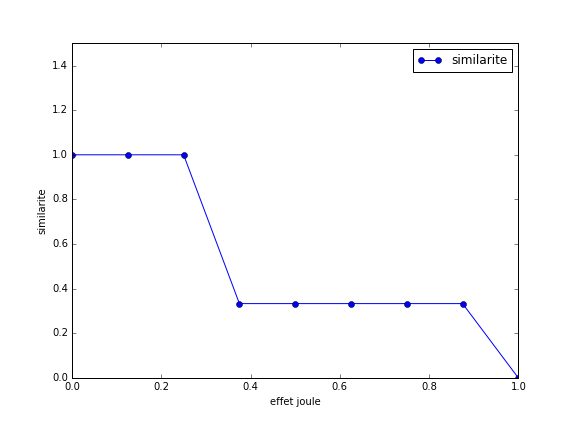
\includegraphics[scale=0.50]{courbe_similarite_selon_EJ_pour_epsilon_075.png}
\caption{ Le coefficient de similarit\'e en fonction des pertes par {\em effets joules} pour $epsilon=0.75$.}
\label {courbeEJCoef}
\end{figure}
\FloatBarrier

%experience 2
\paragraph{exp\'erience 2} :
Ici, on suppose la similarit\'e \'egale \`a $1$ et on cherche les variations de la variable $\epsilon$ en fonction des pertes par {\em effets joules}. 
Les pertes par {\em effets joules} varient de $[0,1]$ par pas de $0.125$ et nous distinguons $8$ intervalles [0,0.125], ]0.125,0.250], ]0.250,0.375], ]0.375,0.5], ]0.5,0.625], ]0.625, 0.75], ]0.75,0.875], ]0.875,1]. 
Pour chaque valeur $\epsilon$, on compte les intervalles $EJ_x, x \in [1,8]$ dans lesquelles la similarit\'e est \'egale \`a $1$ not\'e $X(\epsilon)$. Ainsi $X(\epsilon=0.3) = 8$ signifie que  les pertes par effets joules varient de $0$ \`a $1$ (EJ=[0,1]) et $X(\epsilon=0.3) = 2$ correspond \`a une variation de $EJ$ sur l'intervalle $[0,0.250]$.
On cr\'ee ainsi la distribution de $\epsilon$ en fonction des pertes par effets joules.
La figure \ref{courbeEpsilonEJ}  r\'esume cette distribution qui varie de $1$ (correspondant \`a une variation sur [0,0.125]) \`a $8$ (correspondant \`a une variation sur [0,1]).
La courbe de cette distribution est constante de l'intervalle $\epsilon = [0,0.125]$ puis  d\'ecroissante de l'intervalle $\epsilon =[0.125,1]$ et cette pente est tr\`es accentu\'ee dans l'intervalle $\epsilon = [0.8, 1]$. 
Au d\'el\`a  de $\epsilon > 0.8$, les pertes par effets joules varient dans l'intervalle $EJ=[0,0.2]$.
On en conclut que le meilleur intervalle est $\epsilon = [0.8, 1]$ pour produire des graphes de similarit\'e \'egale \`a $1$ en pr\'esence de pertes par {\em effets joules} de $20\%$.
\newline
% images
\begin{figure}
\centering
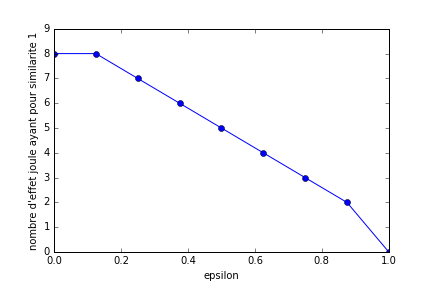
\includegraphics[scale=0.60]{courbe_epsilon_selon_nbreEJ_pour_similarite_1.png}
\caption{ Relation inverse entre $\epsilon$ et $EJ$: $8$ en ordonn\'e correspond \`a $[0,1]$, $7$ \`a $[0, 0.875]$ }
\label {courbeEpsilonEJ}
\end{figure}
\FloatBarrier

% conclusion
{\bf Conclusion} : Ces deux exp\'eriences montrent que la d\'ecision de la fonction {\em Verif-correl}  a une r\'elation inverse avec les pertes par effets joules ($EJ$). En effet, plus $\epsilon$ est petit plus les pertes par effets joules sont grandes et plus les d\'ecisions de {\em Verif-correl} sont erron\'ees.
\begin{equation}
	\epsilon > 1 - EJ
\end{equation}

		\newline 

{\bf Conclusion} :
le r\'eseau \'electrique est mod\'elis\'e par un graphe $G=(V,A,CAP)$.
L'ensemble des sommets $V$ est mod\'elis\'e par des \'equipements sources $V_S$, interm\'ediaires $V_I$ et serveurs $V_C$. Les sous-ensembles  $V_S, V_I, V_C$ sont disjoints deux \`a deux.
Chaque arc $a$ contient des grandeurs physiques $GP^{a}$. Nous en avons denombr\'e $8$ regroup\'ees en 
grandeurs \`a diff\'erentiel de potentiel $gp_{ddp} = \{U_{12}, U_{23},U_{31},U \}$ et en 
grandeurs \`a effet calorifique  $gp_{cal} = \{I_{1}, I_{2}, I_{3}, P \}$.
 Pour chaque grandeur physique $x \in GP^{a}$ associ\'ee \`a l'arc $a$, une capacit\'e $Cap_{a}$ et les mesures $gp_{a}^{x}$ lui sont associ\'ees.
Le flot de mesures $flo$ est un vecteur de mesures qui d\'epend de l'arc $a$, de la grandeur physique $x$ et de la mesure physique $gp_{a}^{x}$. Une valeur de flot $flo_t$  v\'erifie la loi de conservation $R$ et est d\'efinie comme suit :
\begin{equation}
	flo_{t}(a, x, gp_{a}^{x}) = f[a, x, r, cos \phi, gp_{a}^{x}, t] =
	\begin{cases}
		 \frac{  gp_{a}^{x}[t] }{r \times cos \phi}, gp \in \{U, U_{12}, U_{23}, U_{13}  \} \\
		 gp_{a}^{x}[t] , gp \in \{P, Q, I, I_{1}, I_{2}, I_{3}  \}
	\end{cases}
\end{equation}. 
\newline
Nous avons d\'efini la fonction $Verif-correl$, qui \'etant donn\'ee deux ensembles d'arcs $S_1$ et $S_2$, affirme si ces arcs concourent en un sommet $v \in V$ en attribuant  $S_1$ \`a l'ensemble d'arcs entrants et $S_2$ \`a l'ensemble d'arcs sortants du sommet $v$.
Nous consid\'erons que la reponse de $Verif-correl$ est toujours exacte.  

% ----------------------------------------------------------------------------------------------------------------------------------
%		problematique
% ----------------------------------------------------------------------------------------------------------------------------------
	\section{Probl\`eme de d\'ecouverte de topologie \'electrique}
		Notre probl\`eme est de d\'ecouvrir la topologie d'un r\'eseau \'electrique dont on ignore les sommets et on ne connait que les flots dans chaque arc.
% --------- modelisation probleme ===> Donnees
%\subsection{Donn\'ees}
\begin{enumerate}
\item {\bf Donn\'ees} : 
\newline
Nous  avons donc
\begin{itemize}
	\item Un ensemble d'arcs distincts $2$ \`a $2$ du graphe $G$ dont les extr\'emit\'es \textbf{initiales} et \textbf{finales} sont inconnues.\\ $ A =\{ a_{1}, ... , a_{m} \} $ 
		
	\item \`A chaque arc sont associ\'ees des s\'eries de mesures $M(a_{i})$. \\
		$\forall a \in A$, $M(a) = ( gp_{a}^{x})_{x\in GP^{a}}$
		
	\item Chaque s\'erie de mesures $ gp_{a}^{x}$ est de norme $T^{a, x}$ v\'erifiant la remarque de la section ~\ref{remarque},  $x \in GP^{a} \subset GP$
	
	\item $\forall t < T^{a, x}$, $  gp_{a}^{x}[t] $ respecte les r\`egles dans $R$.
\end{itemize}
% --------- modelisation probleme ===> objectif
%\subsection{Objectif}
\item {\bf Objectif} : 
\newline
D\'eterminer la topologie  du graphe $G$ \`a partir des flots des arcs $M(a_{i})$ et des r\`egles $R$ c'est-\`a-dire $\forall a_i$, d\'eterminer $n_1,n_2$ tels que $a_i = (n_1,n_2)$.

% --------- approche
%\subsection{Approche}
\item {\bf Approche} :
\newline
Notre objectif est de d\'eduire la topologie du r\'eseau \'electrique repr\'esent\'ee sous la forme d'un graphe de flots. Notre approche se subdivise en deux \'etapes :
\begin{enumerate}
	\item La premi\`ere \'etape consiste \`a la recherche d'arcs ayant des extr\'emit\'es communes. Pour ce faire, nous calculons la similarit\'e entre les paires de mesures d'arcs pour chaque grandeur dans le but  de d\'eterminer les arcs corr\'el\'es puis nous construirons la matrice de corr\'elation. 
	\item La seconde \'etape est la construction du graphe \`a partir de la matrice de corr\'elation. 
\end{enumerate}


\end{enumerate}
				
% ----------------------------------------------------------------------------------------------------------------------------------
%		 etat de l'art sur la reconstruction/decouverte de reseau
% ----------------------------------------------------------------------------------------------------------------------------------
	\section{\'Etat de l'art sur la d\'ecouverte de topologie}
		Notre probl\`eme de d\'ecouverte de topologie est d'identifier la topologie du r\'eseau \`a partir des mesures c'est-\`a-dire les extr\'emit\'es communes aux arcs dans le r\'eseau.
\newline
Il existe un grand int\'er\^et \`a la d\'ecouverte de topologie notamment dans les syst\`emes distribu\'es avec le d\'eploiement de nouvelles g\'en\'erations de capteurs qui permettent de collecter des mesures selon diff\'erentes granularit\'es (millisecondes, secondes, minutes, quart d'heure, etc).
La communaut\'e scientifique examine tr\`es peu comment interpr\'eter ces mesures et l'impact de celles-ci dans le r\'eseau.
En effet, beaucoup de travaux sont orient\'es sur la d\'ecouverte de la topologie au moyen de protocoles r\'eseau. Des sondes sont propag\'ees dans le r\'eseau omettant la pr\'esence de capteurs dans les r\'eseaux. D'autres travaux cherchent \`a pr\'edire la topologie du r\'eseau informatique \`a partir des lois statistiques et des mod\`eles de files d'attentes.
\newline
Nous regroupons ces travaux en troix axes.
Les deux premiers axes font principalement de la m\'etrologie et cela leur permet de d\'eduire la topologie en connaissant les caract\'eristiques de chaque lien et de chaque n\oe ud du syst\`eme.
Le dernier axe porte sur la reconstruction de la topologie par les s\'eries temporelles.

\subsection{D\'ecouverte des topologies par des sondes}
La d\'ecouverte de topologie est un sujet important dans les r\'eseaux informatiques.
En effet, dans ces r\'eseaux,  on connait la topologie physique et les n\oe uds mais on ignore l'\'etat des n\oe uds. On recherche alors la topologie fonctionnelle du r\'eseau (l'interconnexion entre les n\oe uds) selon l'\'etat des n\oe uds. 
Il existe de nombreux outils pour sonder et faciliter les t\^aches d'administration de ces r\'eseaux. 
Ces outils permettent aux administrateurs r\'eseau de manager efficacement et de d\'ecouvrir le r\'eseau.
Nous citons HP OpenView \cite{OpenView} capable de localiser une erreur et d'envoyer des notifications de plusieurs \'ev\`enements. Ces \'ev\`enements incluent principalement des pertes dans le r\'eseau et les informations sur les caract\'eristiques des liens.
L'inconv\'enient de ces outils est leur co\^ut et ils ne sont pas abordables pour les petites et moyennes organisations.
La d\'ecouverte de r\'eseaux informatiques s'effectue  aussi avec des protocoles r\'eseaux dont les plus connus sont ICMP \cite{rfc792} et SNMP \cite{rfc2821}.
Divers algorithmes ont \'et\'e propos\'es. 
Nous pouvons citer l'algorithme de {\em Narayan et al.} \cite{Breitbart:2004:TDH:1008463.1008464} qui r\'ealise la d\'ecouverte de topologie et de services pour des r\'eseaux h\'et\'erog\`enes en se servant du syst\`eme netInventory \cite{breitbart2004topology}. 
Cet algorithme est bas\'e sur deux hypoth\`eses : 
$(i)$ chaque domaine doit avoir un seul sous-r\'eseau et 
$(2i)$ les tables de routage sont compl\`etes. 
Pour la d\'ecouverte de topologie, le syst\`eme {\em netInventory} \'enum\`ere la liste des adresse IP, envoie des messages ECHO ou ICMP pour d\'eterminer si un n\oe ud est actif. Dans le cas o\`u PING est d\'esactiv\'e, netInventory se sert de ipRouteTable et ipNetToMediaTable dans les routeurs pour connaitre l'\'etat d'un n\oe ud.
\newline
De m\^eme, l'algorithme propos\'e par {\em Kuangyu Qin} \cite{QinKuangyuChunquan2010} est bas\'e sur {\em SNMP} et suppose que l'administrateur r\'eseau est connect\'e \`a l'interface de routage et envoie des paquets de d\'ecouverte aux routeurs. La station de gestion d\'ebute la d\'ecouverte par la lecture des tables de routage. En utilisant les MIB (Management Information Base) et les agents SNMP, cet algorithme \'elimine les \'equipements redondants et g\'en\`ere une topologie efficiente m\^eme quand il existe des VLAN dans le r\'eseau.
\newline
Un autre algorithme, propos\'e par {\em Bilal Saeed, TarekSheltami et Elhadi Shakshuki} \cite{SAEED2015104}, est bas\'e sur netInventory et acc\'el\`ere la d\'ecouverte de la topologie sans g\'en\'erer un trafic suppl\'ementaire. Cet algorithme, nomme TDA (Topology Discovery Algorithm), se sert de la programmation parall\`ele pour g\'erer toutes les requ\^etes de d\'ecouverte des interconnexions r\'eseaux sur la plateforme Android.
Une \'etude bibliographique, effectu\'ee par {\em Ahmed et al.} \cite{AhmedRafatAbouchabaka2014}, fournit les diff\'erentes techniques et algorithmes pour la d\'ecouverte de topologie de r\'eseaux informatiques. Les auteurs d\'eclarent que la plupart des algorithmes de d\'ecouverte de topologie physique de r\'eseau sont bas\'es sur le protocole SNMP. En d'autres termes, ils supposent que tous les n\oe uds de ce r\'eseau sont repertori\'es et activ\'es au moment de la d\'ecouverte. 
\newline

{\bf Conclusion} :
cette m\'ethode est contraire \`a notre sujet de recherche dans lequel nous ignorions les n\oe uds de notre r\'eseau.

\subsection{Tomographie des r\'eseaux}
La tomographie de r\'eseaux est une m\'ethode qui \'etudie les caract\'eristiques internes d'un r\'eseau (c'est-\`a-dire les liens et n\oe uds ON/OFF, la bande passante, la congestion du r\'eseau) en utilisant les mesures point-\`a-point (entre n\oe uds) obtenues \`a partir des sondes plac\'ees dans ce r\'eseau et en supposant que le r\'eseau est mod\'elisable (on peut d\'efinir un mod\`ele avec l'estimateur du maximum de vraisemblance ou l'inf\'erence bay\'esienne). Il fait aussi la pr\'ediction de la topologie du r\'eseau.
\newline
Cette m\'ethode est utilis\'ee en l'absence de syst\`eme de supervision fiable pour identifier les caract\'eristiques des liens et faire un diagnostic de ce dernier (quel n\oe ud/lien est indisponible, congestionn\'e ou ajout\'e) car il est impossible de contr\^oler les flux et l'\'etat des \'equipements.
Les probl\`emes, r\'esolus par la tomographie des r\'eseaux,  sont regroup\'es en $3$ cat\'egories :

\subsubsection{L'estimation des param\`etres (caract\'eristiques) d'un lien}

L'article de {\em Ghita et al.} \cite{ghitaArgyrakiThiran2010} se propose de d\'ecouvrir la congestion des liens dits "corr\'el\'es" dans un r\'eseau informatique.
Un lien entre deux n\oe uds du r\'eseau est une connexion logique au niveau de la couche $3$ du protocole TCP/IP et deux liens sont corr\'el\'es s'ils appartiennent au m\^eme domaine ou sous-r\'eseau.
Pour r\'ealiser cet algorithme, il consid\`ere que la topologie du r\'eseau et le degr\'e de corr\'elation entre les liens sont connus et qu'il existe un trafic unicast entre les n\oe uds dans le r\'eseau (ce trafic est d\'esign\'e par chemin).
Il \'enonce quatre hypoth\`eses pour l'exp\'erimentation de l'algorithme : 
$(i)$ l'ensemble des chemins reste inchang\'e durant chaque simulation; 
$(2i)$ chaque chemin est congestionn\'e si au moins un lien du chemin est congestionn\'e; 
$(3i)$ le comportement de congestion de chaque lien pendant chaque simulation est mod\'elis\'e par un processus al\'eatoire stationnaire; 
$(4i)$ deux ensembles de corr\'elations disjoints ne doivent pas \^etre travers\'es par les m\^emes chemins.
\newline
Diff\'erentes m\'ethodes ont \'et\'e propos\'ees et valid\'ees mais elles diff\`erent de l'algorithme {\em Ghita et al.} \cite{ghitaArgyrakiThiran2010} par les caract\'eristiques des liens fournis.
En effet, les m\'ethodes initiales se basent sur les corr\'elations temporelles, chacune parfaitement corr\'el\'ee et envoy\'ee par des packets multicast \cite{adamsBuFreidmanHorowitz2000, aryaDuffieldVeitch2008, buDuffieldPrestiTowsley2002, caceresDuffieldHorowistzTowsley1999}. 
Tous les taux de pertes des liens sont statistiquement identifiables dans une topologie en arbre \cite{chenCaoBu2007}.
Cependant le multicast n'est pas largement d\'eploy\'e et les groupes de paquets unicast exigent un d\'eveloppement subtantiel et un co\^ut d'administration \'elev\'e. D'o\`u il est moins ais\'e de s\'electionner les corr\'elations temporelles.
\newline
L'ensemble des m\'ethodes qui suivent \cite{nGDuffield2006, padmanabhanQiuWang2003,sommerBarfordDuffieldRon2007, zhaoChenBindel2006} utilisent seulement des mesures unicast point-\`a-point (c'est-\`a-dire des mesures sur les liens) dans le simple but d'identifier les congestions de liens.
\newline
Les m\'ethodes bool\'eennes de tomographie de r\'eseaux consid\`erent des hypoth\`eses suppl\'ementaires \cite{padmanabhanQiuWang2003,nGDuffield2006} pour identifier les liens congestionn\'es en trouvant le plus petit ensemble de liens qui peut \^etre expliqu\'e par ces mesures.
Ces hypoth\`eses sont : 
$(i)$ les liens sont ind\'ependants;
$(2i)$ les liens sont congestionn\'es \'equiprobablement; 
$(3i)$ le nombre de liens congestionn\'es est faible.
Toutes les pr\'ec\'edentes m\'ethodes \cite{ghitaArgyrakiThiran2010, nGDuffield2006, padmanabhanQiuWang2003,sommerBarfordDuffieldRon2007, zhaoChenBindel2006} se basent sur l'ind\'ependance des liens c'est-\`a-dire l'hypoth\`ese $(i)$.

\vspace{-0.4cm}  
\subsubsection{La pr\'ediction de topologie} 

L'objectif de cette m\'ethode est d'identifier l'arbre de la topologie connectant un serveur aux autres machines du r\'eseau.
L'id\'ee est d'utiliser une fonction croissante (ou monotone) du nombre de liens partag\'es entre deux n\oe uds ou le maximum de vraisemblance pour trouver l'arbre.
\newline
L'article de {\em Coates and al.} \cite{coatesCastroNowak2002} suppose que les mesures de la couche $2$ (protocole TCP/IP) des machines clientes sont assez fiables pour d\'ecouvrir le r\'eseau. Les mesures sont collect\'ees \`a l'aide de l'outil Traceroute. Ensuite l'auteur d\'efinit un mod\`ele bas\'e sur les chaines de Markov de Monte Carlo pour d\'eterminer les caract\'eristiques des liens du r\'eseau et d\'eduire les topologies probables. Enfin il propose un crit\`ere global du seuil maximum pour l'identification de topologie contrairement aux autres travaux \cite{andrieuDoucetFitzgerald2000bayesian, bestavrosAzerByers2005inference} qui emploient des strat\'egies semi-optimales de fusion des liens.
 
\subsubsection{La densit\'e du trafic entre \'emetteur/recepteur}

 Un probl\`eme de tomographie de r\'eseaux qui retient notre attention est l'estimation de la matrice de trafic qui pr\'evoit le volume de flots entre les n\oe uds point-\`a-point \`a partir des mesures \cite{vardi1996, caoDavisWielYu2000}.
En effet, les variables inconnues sont les volumes de flots et nous suivons une certaine loi de probabilit\'e.
\newline
Les corr\'elations de flots ont \'et\'e \'etudi\'ees par {\em Singal et Michailidis} \cite{singalMichailidis2007} et ils montrent que, sous certaines classes de d\'ependances, les moments d'ordre $n$ de ces volumes de flots sont identifiables \`a partir des mesures de liens pour $n \ge 2$.
Cette approche diff\`ere de $2$ aspects par rapport \`a l'estimation des caract\'eristiques de liens.
Premi\`erement, l'estimation des caract\'eristiques s'int\'eresse aux mesures point-\`a-point c'est-\`a-dire sur les liens tandis que le calcul du trafic point-\`a-point doit \^etre estim\'e dans la densit\'e de trafic \cite{vardi1996, singalMichailidis2007, caoDavisWielYu2000}.
Deuxi\`emement, l'estimation des caract\'eristiques utilise les variables bool\'eennes et la connaissance des valeurs des variables des lois de distributions n'est pas n\'ecessaire comme cela se fait dans la densit\'e de trafic. La connaissance des valeurs des param\`etres engendre la restriction de l'extension des r\'esultats th\'eoriques \cite{singalMichailidis2007}.
\newline

{\bf Conclusion} :
la tomographie de r\'eseaux n'est pas appropri\'ee pour notre sujet de recherche car nos mesures d'arcs d\'eterminent les caract\'eristiques de ces arcs et les n\oe uds sont inconnus emp\^echant la d\'ecouverte de r\'eseau qui est l'\'etape n\'ecessaire pour d\'ebuter la tomographie de r\'eseaux.


\subsection{Reconstruction de la topologie par les s\'eries temporelles}
Le brevet de {\em Chaudhary et al.} \cite{chaudhary2016network} d\'ecrit comment trouver le graphe induit par un r\'eseau de canalisations de fluides en se servant des mesures de capteurs de diff\'erentes stations qui \'emettent des fluides. Il consid\`ere le r\'eseau comme un arbre dans lequel la racine est une station comprenant un compresseur. La pr\'esence du compresseur induit un d\'elai de livraison entre la station source et les stations de livraison (d\'elai d'acheminement du fluide entre les n\oe uds du r\'eseau). 
Le d\'elai est d\^u au temps mis par le fluide pour atteindre la station de livraison. 
\newline
Le traitement des mesures \cite{cincotta1995astronomical, hurley2011methods, mohanty2000robust} porte sur la recherche de pics, la suppression d'anomalies (observations non conformes \`a un motif dans le dataset de donn\'ees) et le lissage des donn\'ees. 
Les donn\'ees obtenues identifient la relation d'adjacences entre les n\oe uds.
Le traitement des retards temporels d\'eterminent la distance entre des n\oe uds du r\'eseau.
L'analyse des s\'eries temporelles par paires d\'etermine la causalit\'e entre les capteurs associ\'es. 
La causalit\'e est la recherche d'\'ev\`enements identiques observ\'es dans deux s\'eries de mesures.
En d'autres termes, la causalit\'e consiste \`a savoir si les \'ev\`enements, observ\'es dans une s\'erie de mesures, se reproduisent dans une autre s\'erie. 
Un mod\`ele de causalit\'e bas\'e sur les s\'eries temporelles des stations est d\'efini comme une r\'egression multiple avec un mod\`ele de Granger.
\`A partir de ce mod\`ele, on calcule les diff\'erents retards $X(t)$ et leurs coefficients.
On d\'efinit \'egalement un mod\`ele de p\'enalisation bas\'e sur une r\'egression LASSO afin de filtrer les relations de causalit\'e et obtenir un graphe creux (sparse). 
Le graphe de causalit\'e est alors un arbre.
\newline
Les auteurs {\em Chaudhary et al.}  proposent un script s'ex\'ecutant r\'ecursivement sur les n\oe uds du r\'eseau en choisissant, \`a chaque \'etape, les n\oe uds qui ne sont pas des puits. En se servant du graphe de causalit\'e (corr\'elation) et des retards de propagation, il d\'etermine les voisins du n\oe ud $X_i$ et supprime les n\oe uds voisins de $X_i$  ayant une causalit\'e entre eux car le r\'eseau est un arbre.
\newline
La m\'ethode d\'ecrite ici est la construction du graphe it\'erativement \`a partir des sous-arbres du graphe. 
En effet, le nombre de sous-arbres est l'ordre dans lequel on a supprim\'e les n\oe uds puits. 
Cette m\'ethode est r\'ealisable en $O(n^2)$ car chaque sommet est trait\'e une fois et la recherche de son voisinage est en $O(n)$ avec $n$ le nombre de sommets.
\newline 
Cette m\'ethode est inadapt\'ee pour un DAG car sa complexit\'e est en $O(n^n)$.
Elle ne s'ex\'ecute que sur des arbres.
\newline
		\newline
{\bf Conclusion} :
l'\'etude bibliographique effectu\'ee sur la d\'ecouverte de topologie montre que la recherche sur ce sujet  est tr\`es active dans le domaine des r\'eseaux informatiques, pr\'ecisement dans la d\'etection de n\oe uds/liens congestionn\'es. 
Toutefois, dans le domaine \'energ\'etique, les rares travaux r\'ealis\'es sur ce sujet mettent l'accent sur la d\'ecouverte de topologie par la reconstruction des sous-graphes en supposant que les n\oe uds du r\'eseau sont connus, 
que certains liens sont absents, 
que les mesures sont influenc\'ees par les incidents 
et que des erreurs peuvent \^etre pr\'esentes sur nos donn\'ees. 
Ces travaux s'av\`erent moins pertinents pour notre probl\'ematique parce  que les r\'esolutions propos\'ees s'appuyent sur des hypoth\`eses qui sont diff\'erentes des n\^otres. 
En effet, nous connaissons que les liens et les mesures qui circulent sur ces liens. 
Mais nous ignorons exactement les extr\'emit\'es de ces liens.
Par ailleurs, ces mesures suivent  des lois physiques qui impliquent la propagation d'\'ev\`enements dans ces r\'eseaux.
Notre probl\'ematique est alors de d\'eterminer les extr\'emit\'es partag\'ees entre les liens  gr\^ace aux lois et aux mesures physiques et aussi \`a la th\'eorie des graphes.


	
			
% ----------------------------------------------------------------------------------------------------------------------------------
%		 conclusion
% ----------------------------------------------------------------------------------------------------------------------------------
	\section{Conclusion du chapitre \ref{ReseauFlotsMesures}}
		Dans ce chapitre, nous avons montr\'e que 
le r\'eseau \'electrique se mod\'elise par un graphe de flots dont les sommets sont des \'equipements, les arcs sont les c\^ables \'electriques unidirectionnels et les flots par les mesures des \'equipements. Par convention, ces mesures sont port\'ees par les arcs incidents entrants dans chaque sommet du graphe. 
Chaque mesure est associ\'ee \`a une grandeur physique et \`a chaque grandeur est d\'efinie une capacit\'e sur l'arc. Nous avons red\'efini la loi de conservation $R$ en fonction de nos mesures,  de nos grandeurs et nos capacit\'es.  
\newline
%Dans ce graphe, les arcs et leurs flots sont connues mais les sommets sont inconnues. Notre probl\`eme est de d\'eterminer les sommets communs aux arcs.
Dans ce graphe, nous connaissons les liens et les mesures qui circulent sur ces liens. 
Mais nous ignorons exactement les extr\'emit\'es de ces liens.
Par ailleurs, ces mesures suivent  des lois physiques qui impliquent la propagation d'\'ev\`enements dans ces r\'eseaux.
Notre probl\`eme est alors de d\'eterminer les extr\'emit\'es partag\'ees entre les liens  gr\^ace aux lois $R$, aux mesures physiques et aussi \`a la th\'eorie des graphes.
\newline
Une \'etude bibliographique a \'et\'e r\'ealis\'ee sur la d\'ecouverte de topologie. Les travaux concernent principalement la reconstruction de topologie dans le domaine informatique \`a partir de sondes et de protocoles de r\'eseau. Ces travaux s'accentuent sur la supervision de r\'eseau, l'administration du r\'eseau et aussi sur la recherche des caract\'eristiques des \'el\'ements du r\'eseau. 
Dans le domaine \'energ\'etique, nous avons trouv\'e un brevet qui reconstruit des sous-graphes du r\'eseau \`a partir de la propagation des incidents.
Tous ces travaux supposent que nous connaissons l'\'etat de tous les \'el\'ements du r\'eseau. Ce qui est contraire \`a notre probl\'ematique.
\newline
 Nous avons propos\'e deux approches pour r\'esoudre notre probl\`eme. La premi\`ere approche consiste \`a d\'eterminer la corr\'elation entre les arcs \`a partir des mesures et des r\`egles de flots puis \`a construire une matrice de corr\'elation. La seconde approche d\'ecouvre le r\'eseau en effectuant certaines transformations sur la matrice de corr\'elation.  

		